\section{Métodos}
\subsection{Amplificação dos Lasers Raman}

A frequência de Rabi de uma transição atômica de dois fótons é dada por 
\begin{equation}
    \Omega = \frac{\Omega_1\Omega_2}{2\Delta}
\end{equation}
Onde $\Omega_i=-2\frac{\mathbf d \cdot E_i}{\hbar} \propto \sqrt I_i$ é a frequência de Rabi de cada laser e proporcional à raiz quadrada de sua intensidade. $\mathbf d$ é o dipolo dos átomos e $\Delta$ é o desacordo escolhido para ser em torno de \SI{1}{GHz} para evitar a emissão espontânea. 
Para implementar o interferômetro Raman nos átomos em queda livre, precisamos de uma frequência de Rabi de cerca de \SI{50}{kHz}, o que não foi alcançado com a configuração anterior (que era dedicada à realização de um interferômetro atômico aprisionado). Portanto, uma amplificação do nosso laser é necessária \cite{cheinet2006conception}. Uma maneira conveniente de aumentar a potência de um laser de diodo sem alterar as propriedades espectrais e de coerência da luz é usar um amplificador em forma de cone (\gls{TA}). O chip \gls{TA} com as lentes de entrada e saída está fixado em um suporte de cobre, que é mostrado na figura \ref{fig:mount} junto com sua configuração óptica.

\begin{figure}
    \centering
    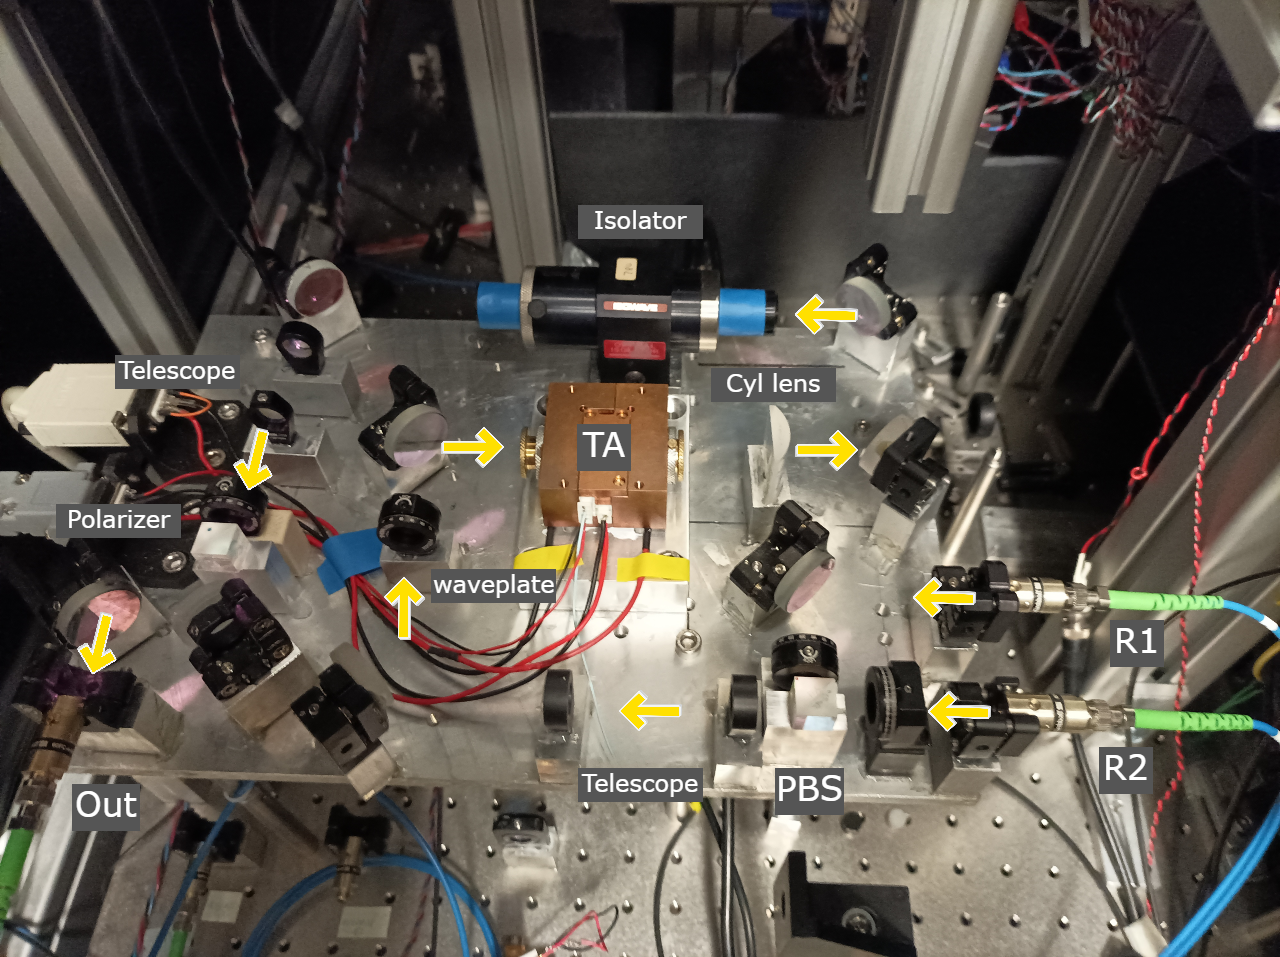
\includegraphics[width=0.7\linewidth]{figures/TA-mount-labels.png}
    \caption{O módulo laser usado para amplificação de luz desenvolvido durante o estágio.}
    \label{fig:mount}
\end{figure}

\subsubsection{Injeção dos Lasers Raman}
Os feixes (R1 e R2 na figura \ref{fig:mount}) necessários para a excitação Raman dos átomos têm um comprimento de onda em torno de \SI{780}{nm}. Ambos os feixes saem de fibras ópticas monomodo com manutenção de polarização e foram sobrepostos e amplificados no mesmo setup.

Para alinhá-los, utilizou-se um cubo \gls{PBS} juntamente com placas de onda de $\lambda /2$ para cada feixe antes do cubo. O cubo \gls{PBS} atua como um polarizador, refletindo ou transmitindo uma certa quantidade do laser dependendo de sua polarização (em vez de absorver a parte que não está alinhada como um polarizador comum). O divisor de feixes também redirecionará os dois feixes na mesma direção com polarizações diferentes e ortogonais, pois um dos feixes foi transmitido e o outro foi refletido.

Para ajustar a colimação dos dois feixes sobrepostos, usamos um telescópio com duas lentes com comprimentos focais idênticos.

\subsubsection{Amplificador Tapered (TA)}
O \gls{TA} é um chip semicondutor de meio de ganho laser sem cavidade. Portanto, quando um feixe de laser passa por ele, é amplificado. A face de entrada do TA tem um tamanho de alguns \si{\micro m}. Assim, é necessário focar o feixe de entrada precisamente nessa área. Devido à forma do chip TA, seu modo de saída natural é astigmático, o que significa que ele diverge nas direções horizontal e vertical com diferentes comprimentos focais. O \gls{TA} escolhido para a montagem do experimento é o amplificador óptico semicondutor de \SI{780}{nm} do modelo EYP-TPA-0780-01000-3006-CMT03-0000 da empresa Toptica Eagleyard. O amplificador também necessita de um regulador de temperatura, que é externo a ele.

O chip TA, semelhante a um diodo laser, precisa de uma corrente para bombear seu meio em uma inversão de população para atuar como um meio de ganho. No setup, usamos uma fonte de corrente comercial Thorlabs LDC220C, que pode ser ajustada de \SI{0}{mA} a \SI{2000}{\mA} para este \gls{TA}. Enquanto estava sendo alinhado e ajustado, a corrente foi reduzida para \SI{700}{mA} por motivos de segurança do laser. Mas, como a corrente usada no experimento será em torno de \SI{1500}{mA} e o modo do feixe de saída resultante pode mudar com a corrente no \gls{TA}, o acoplamento de fibra foi otimizado para essa corrente. Potências acima de \SI{500}{mW} foram medidas com um medidor de potência térmica.

O eixo de polarização do feixe de entrada do \gls{TA} deve estar alinhado ao eixo lento da fibra PM do amplificador tapered. Mas, como mencionado na seção anterior, a polarização dos dois feixes é ortogonal quando combinados no \gls{PBS}. Assim, inserimos uma placa de onda de meia onda antes da entrada do TA para girar ambas as polarizações até encontrarmos um compromisso entre as potências de saída dos dois feixes. Para encontrar esse compromisso, tracei o ângulo da placa de onda e a potência resultante para os 2 feixes. E então escolhi o ângulo da placa de onda onde os dois se encontram com a maior potência (veja a figura \ref{fig:compromise}).

\begin{figure}
    \centering
    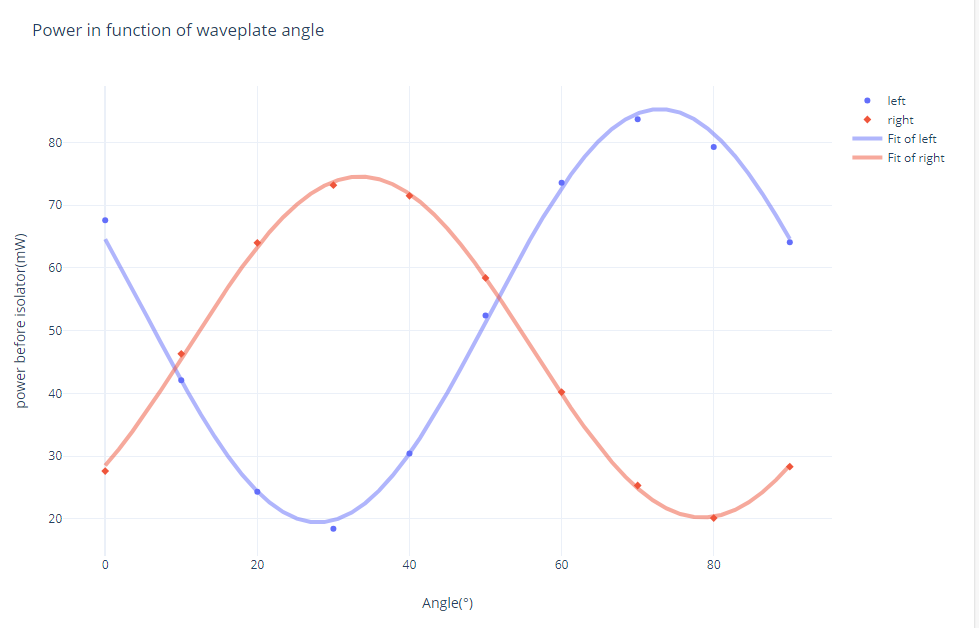
\includegraphics[width=0.5\linewidth]{figures/non_normalized_waveplate.PNG}
    \caption{Ângulo da placa de onda vs potência dos 2 feixes}
    \label{fig:compromise}
\end{figure}

Acoplamos os feixes de entrada no \gls{TA} com a ajuda de seu \gls{ASE} de retrocedente. Este \gls{ASE} é emitido naturalmente do TA através de ambas as extremidades quando o \gls{TA} é acionado por uma corrente. Para ajustar as lentes que focam a entrada no chip \gls{TA}, podemos colimar o feixe \gls{ASE} de retrocedente que sai da entrada.  
Então, podemos sobrepor o \gls{ASE} retrocedente na entrada com os feixes de entrada.

Outro requisito importante para maximizar a saída do \gls{TA} é a colimação dos feixes de entrada. No nosso caso, as posições das lentes de colimadores de entrada se moveram ao transferir o módulo para o laboratório, e tivemos que corrigir isso para recuperar o nível adequado de potência novamente.

\subsubsection{A saída do \gls{TA}}
Na montagem do \gls{TA}, podemos inserir uma lente esférica (com comprimento focal de \SI{3,1}{mm}) para colimar verticalmente o feixe na direção de saída. Como o feixe é astigmático, a outra direção não será colimada. Para colimar a direção horizontal, usamos uma lente cilíndrica (com comprimento focal de \SI{38,1}{mm}). Devido ao pequeno tamanho do chip TA, é difícil alinhar corretamente e, em particular, ajustar sua posição em seu suporte na altura ideal. Por esse motivo, a direção do feixe de saída acabou sendo ligeiramente inclinada em relação ao eixo óptico da montagem do \gls{TA}. Como nossa lente cilíndrica foi colocada diretamente após o \gls{TA}, essa inclinação causou aberrações significativas no feixe resultante, o que reduziu a eficiência de acoplamento na fibra monomodo mais adiante. Também tivemos algumas aberrações devido à lente esférica montada no amplificador por causa dessa inclinação. Isso demonstra a importância de um suporte preciso do chip \gls{TA} ao construir o \gls{TA}.

\subsubsection{Isolador Óptico}
Se um dos componentes ópticos no caminho óptico refletir alguma luz de volta, ela pode acoplar no \gls{TA} e interferir em seu funcionamento. O mesmo pode acontecer com o laser de acionamento do \gls{TA}. Isoladores ópticos são usados para prevenir a propagação de luz do laser de volta. Um isolador óptico age como uma válvula ou diodo, mas para luz polarizada. É composto por um polarizador vertical na entrada, seguido por um rotador de Faraday que usa um campo magnético para girar a luz passando \ang{45} e outro polarizador a \ang{45} na saída. A luz que entra passa verticalmente, é girada \ang{45} e passa pelo segundo polarizador. Mas a luz que vem da direção oposta é girada para horizontal e não consegue passar pelo polarizador vertical na entrada. Assim, é bloqueada.

Na nossa montagem, usamos o modelo Isowave I-80-T4 H. Acoplamos com dois espelhos de ajuste após a lente cilíndrica. Após ajustar o isolador, ele estava refletindo alguma luz de volta para o \gls{TA}, o que levou a oscilações de potência com um período de \SI{250}{s}. Tivemos que inclinar o isolador alguns graus para que o laser refletido não acoplasse no amplificador enquanto o feixe principal ainda passava pelo isolador.

\subsubsection{Acoplamento da fibra de saída}
Logo após o isolador, temos um espelho desviando o feixe para dois outros espelhos de ajuste para acoplar o feixe na fibra de saída. Apesar de ajustar a lente colimadora, inicialmente só conseguimos uma eficiência de acoplamento muito baixa de \SI{10}{\percent}-\SI{15}{\percent} em comparação com a potência antes do colimador.

Usamos uma câmera perfiladora de feixe para visualizar o perfil do feixe do TA logo após o isolador, bem como um feixe saindo da fibra de saída. Excluindo as aberrações, a largura gaussiana do feixe amplificado era cerca de \SI{3,5} vezes menor que a largura do feixe do colimador para a fibra dada. Portanto, colocamos um telescópio antes dos espelhos de ajuste com lentes de \SI{-15}{mm} e \SI{50}{mm} para aumentar o feixe e combinar o modo da fibra. Dessa forma, quase dobramos nossa eficiência de acoplamento para \SI{25}{\percent}, que ainda é uma eficiência bastante baixa, causada pelas aberrações do perfil do feixe devido à montagem do \gls{TA}.

Para estabilizar a polarização acoplada na fibra, adicionamos um \gls{PBS} e uma placa de onda de meia onda antes da fibra (veja a figura \ref{fig:mount}).

\subsubsection{Transferência do setup para o experimento}
Quando o módulo foi colocado no lugar no experimento, alguma luz do \gls{TA} estava voltando e interferia com um dos lasers de diodo, o que levou a um feedback óptico, embora o laser já estivesse equipado com um isolador. Esse problema foi resolvido colocando um isolador adicional no laser.

\subsection{Trava de Fase de R1 em R2}
Na transição Raman, é importante que a fase do laser e sua diferença de frequência sejam consistentes; por isso, fazemos a trava de fase, que também trava a diferença de frequência entre eles (em \SI{6,834}{GHz}, veja a figura \ref{fig:levels}). Um sinal que codifica essa diferença é gerado por uma fotodiodo, que registra a frequência da batida entre os dois lasers. A frequência da batida, que é igual à diferença de frequência entre eles, é reduzida por mistura com um sinal de referência de micro-ondas. A frequência de RF resultante é comparada com o sinal de um DDS em um detector de frequência de fase. O sinal de erro de fase é então usado para travar a fase dos lasers, corrigindo a corrente do laser de R1 e também o comprimento da cavidade externa através de um atuador piezoelétrico.

A trava de fase para esses lasers já estava implementada no experimento. O nível da nota de batida deve estar na faixa de \SI{-50}{dBm} a \SI{-30}{dBm} e pode ser verificado com um analisador de espectro.

\subsection{Trava de Offset de R2 no laser de Repump}
A trava de offset funciona de maneira semelhante à trava de fase. No entanto, usamos a batida para corrigir apenas a frequência de um dos lasers Raman. O objetivo de manter a frequência deste laser estável é evitar que o desacordo $\Delta$ de cerca de \SI{1}{GHz} do estado intermediário da transição Raman derive. A deriva sem a trava é da ordem de centenas de Megahertz e, portanto, significativa. O ponto de trava para a configuração atual (deslocado para o vermelho) é uma nota de batida de \SI{900,8}{MHz}.

A fotodiodo para esta trava foi inserida em um mini-circuit bias-tee. O bias-tee é alimentado por uma bateria de \SI{9}{V}. Ao observar uma pequena tensão nos terminais da bateria desconectados, obtemos um sinal quando há um laser na fotodiodo. Fazendo isso, podemos alinhar os lasers com a fotodiodo otimizando a tensão nesses terminais.

Para sobrepor os dois feixes, usamos um \gls{PBS}s e placas de onda para redirecionar parte dos dois feixes a serem travados na fotodiodo. Como suas polarizações eram ortogonais, para obter a mesma polarização, usamos um \gls{PBS} girado em \SI{45}{\degree}. Uma lente de comprimento focal de \SI{25}{mm} foi adicionada no caminho para focar o laser na pequena abertura da fotodiodo (veja a figura \ref{fig:lock_optics}).

\begin{figure}
    \centering
    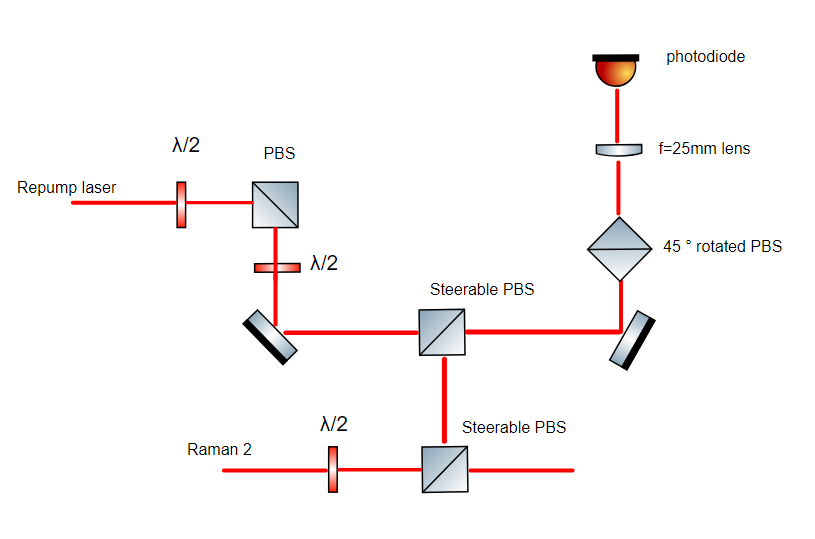
\includegraphics[width=0.5\linewidth]{figures/lock_optics.PNG}
    \caption{Configuração óptica para a trava de offset do laser.}
    \label{fig:lock_optics}
\end{figure}

A nota de batida vai do bias-tee para um amplificador, para um acoplador direcional, e então para um conversor F-U. O F-U é uma caixa que converte uma frequência de sinal em uma tensão DC, com uma taxa de conversão linear de \SI{100}{MHz/V}. 
Essa tensão do F-U é então alimentada em um circuito controlador de laser de diodo mostrado na figura \ref{fig:lock_circuit}. 
Esse controlador integra o sinal de erro (entrada \textbf{1} na figura \ref{fig:lock_circuit}), que é a diferença do F-U para uma referência (\SI{9}{V} e entrada \textbf{11}), uma vez para a corrente do laser (em \textbf{5}) e duas vezes para o piezoelétrico (em \textbf{10}).
O loop de frequência é fechado atuando na corrente do diodo laser e no piezoelétrico na cavidade do laser, que controla a frequência do laser. A frequência do laser R2 é então vinculada ao laser de repump, com um offset em frequência. Ao ligar \textbf{3} e \textbf{8}, podemos ativar a trava ou desativá-la para observar o comportamento do laser ou de algum sinal no loop.

\begin{figure}
    \centering
    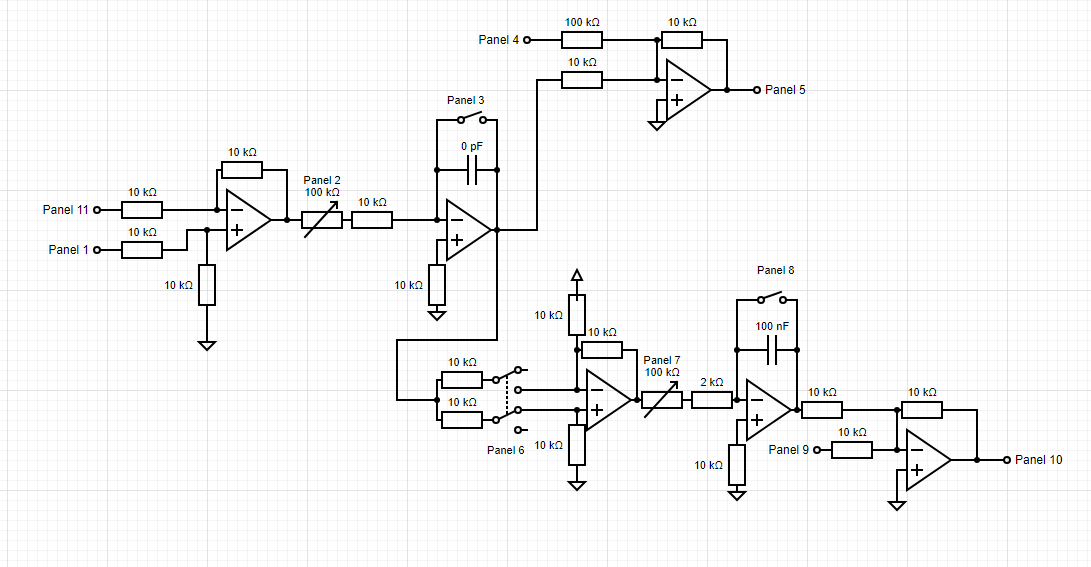
\includegraphics[width=0.9\linewidth]{figures/lock_circuit.png}
    \caption{Circuito para o controlador de laser de diodo da trava de offset. Que controla a corrente do diodo laser e o piezoelétrico da cavidade.}
    \label{fig:lock_circuit}
\end{figure}


\subsection{Estabilização da Potência}
Para o experimento, foi necessário estabilizar a potência dos lasers Raman abaixo de \SI{1}{\percent}. Assim, construímos um controlador para a corrente do \gls{TA} usando a saída de tensão de um fotodiodo. A corrente foi controlada usando a entrada de modulação da fonte de corrente para laser Thorlabs que alimentava o \gls{TA}.

O controlador apenas soma a saída (negativa) do fotodiodo a uma referência e integra esse sinal de erro uma vez. Com a placa de circuito utilizada, podemos alterar facilmente o resistor e a capacitância do integrador. A saída é limitada ao intervalo de \SI{\pm1}{V}. Com o limite ajustado na fonte de corrente Thorlabs de \SI{1550}{mA}, esses \SI{\pm1}{V} equivalem a \SI{\pm155}{mA} quando o controlador está saturado.

Posicionamos um fotodiodo fora do loop antes e depois de um \gls{AOM} e também após um \gls{LCVR}, ambos no caminho do laser antes da câmara de vácuo. Após o \gls{AOM}, medimos um excesso de ruído. Mas após o \gls{LCVR} e um cubo \gls{PBS}, a potência estava ainda mais ruidosa, e a estabilização mal fazia diferença. As flutuações estavam vindo do \gls{LCVR}, que estava perturbando a polarização, o que se convertia em diferenças de potência no \gls{PBS}. Como o \gls{LCVR} não estava mais sendo usado, o removemos.

\subsection{Transições Atômicas}
As variáveis importantes dos lasers Raman para as transições atômicas são: o deslocamento Stark AC, influenciado pela razão de potência entre os dois feixes. A polarização também é crucial, deve ser $\sigma^+$ para ambos, ou linear e perpendicular entre os dois feixes. Finalmente, a frequência de Rabi que é influenciada também pelos desacordos e portanto pelas frequências além das potências dos dois feixes.

\subsubsection{O Deslocamento Stark AC}

Quando os lasers Raman são dirigidos para os átomos, a energia da ressonância com os níveis da transição Raman muda. Isso é chamado de deslocamento Stark AC. O deslocamento varia com a potência, e cada laser terá um deslocamento Stark diferente para a mesma potência e também um deslocamento com sinais opostos. Se houver um deslocamento, átomos em diferentes posições do feixe com diferentes intensidades dos lasers Raman verão deslocamentos Stark AC diferentes, amortecendo a oscilação de Rabi. Portanto, tentamos encontrar uma razão entre os dois lasers onde esse deslocamento seja próximo de zero, como na figura \ref{fig:stark}.

O escaneamento é, em detalhes, um escaneamento do desacordo entre os lasers, que variamos alterando a frequência do sinal de referência de micro-ondas do PLL e, portanto, a diferença no ponto de bloqueio de frequência entre os dois lasers. O mapeamento tem a forma de uma função seno cardinal.

Ao realizar a espectroscopia de micro-ondas da transição hiperfina, na presença de um dos dois lasers, por exemplo, R2, podemos medir o deslocamento Stark AC da transição hiperfina induzido por esse laser. Para R1, obtivemos um deslocamento de \SI{4.5}{kHz} com uma potência medida logo abaixo da câmara de vácuo de \SI{2.6}{mW}, embora este laser estivesse livre e não bloqueado em fase. Para R2, obtivemos \SI{-5.5}{kHz} com uma potência de \SI{0.51}{mW}. Ajustando a razão de potência, pudemos anular o deslocamento diferencial de luz na presença de ambos os lasers, como mostrado na figura \ref{fig:stark}.

\begin{figure}
    \centering
    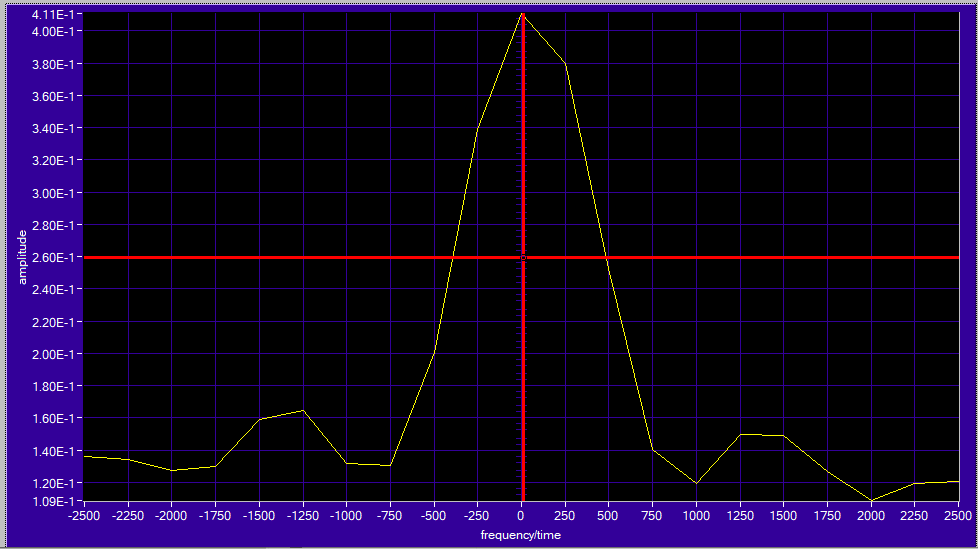
\includegraphics[width=0.5\linewidth]{figures/ResScan11.png}
    \caption{Mapeamento do desacordo entre os feixes Raman nos átomos com deslocamento Stark AC compensado. A frequência está em unidades de \SI{0.1}{kHz}.}
    \label{fig:stark}
\end{figure}

\subsubsection{Picos Contra-propagantes e Co-propagantes}
A figura \ref{fig:prop} exibe o espectro Raman que obtemos, ao escanear a diferença de frequência Raman de um único pulso Raman. Podemos ver que há 3 picos principais em um mapeamento maior de Raman. O do centro é devido às transições Raman co-propagantes, que podem ser vistas apenas com os feixes Raman incidentes, e os dois em \SI{\pm 250}{kHz} que são as transições contra-propagantes e que necessitam do feixe incidente e também da reflexão no espelho no topo da câmara de vácuo, ambos passando pelos átomos. Todos são afetados pelo deslocamento Stark AC e os outros picos menores são apenas os lobos da função sinc.

Ao ajustar a nossa diferença de frequência Raman entre os dois feixes para o deslocamento desses picos, podemos usar a transição co-propagante ou contra-propagante. Como a contra-propagante tem mais transferência de momento, usamos essa configuração para fazer a interferometria de átomos.

\begin{figure}
    \centering
    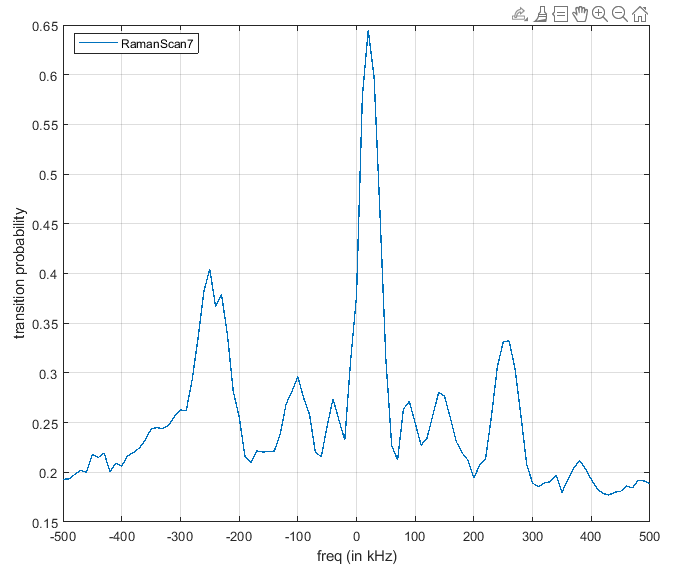
\includegraphics[width=0.5\linewidth]{figures/propagating.png}
    \caption{Mapeamento Raman com picos contra e co-propagantes da transição Raman}
    \label{fig:prop}
\end{figure}

\subsubsection{Oscilações de Rabi}
Quando estamos em ressonância com uma das duas transições contra-propagantes, podemos então induzir oscilações de Rabi, como na figura \ref{fig:rabi}, variando a duração do pulso Raman. Extraímos a partir disso a frequência de Rabi das transições Raman. Podemos usar essa informação para nos posicionar no meio da inclinação crescente no início da oscilação de Rabi. Com isso, somos capazes de otimizar a posição horizontal do feixe Raman nos átomos com uma base de translação, por exemplo. Nesse ponto, com essa duração de pulso, uma potência maior e, portanto, uma frequência de Rabi maior resultaria em uma maior quantidade de átomos no estado excitado. Assim, a cada ciclo, se estamos obtendo mais átomos, significa que temos um melhor alinhamento.

Como não conseguimos alcançar a frequência de acoplamento/Rabi desejada apenas com o aumento da potência do \gls{TA}, reduzimos o desacordo do laser Raman, em detrimento de mais emissão espontânea, para aumentar o acoplamento.

\begin{figure}
    \centering
    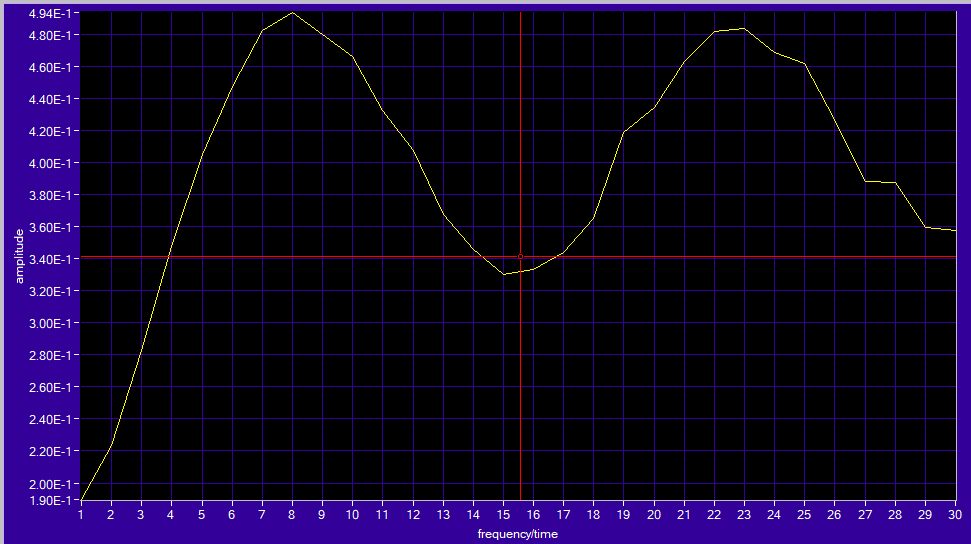
\includegraphics[width=0.5\linewidth]{figures/RabiOsc1.png}
    \caption{Oscilações de Rabi dos átomos sob um mapeamento da duração do pulso dos lasers Raman. As durações dos pulsos no eixo x estão em \si{\micro s}.}
    \label{fig:rabi}
\end{figure}

\section{Resultados}
\subsection{Avaliação de desempenho}
\subsubsection{O \gls{TA}}
Na Tabela \ref{tab:powers}, podemos ver as potências esperadas para \SI{1500}{mA} no \gls{TA} para a entrada do laser dada (que varia com a corrente). Podemos observar que obtemos um aumento significativo nas potências dos lasers acopladas à fibra ao usar o amplificador (veja após a fibra de entrada e após a fibra de saída para comparação).

\begin{table}[]
\begin{tabular}{|p{1.5cm}|p{1.5cm}|p{1.5cm}|p{1.5cm}|p{1.5cm}|p{1.5cm}|p{1.5cm}|}
\hline
Laser & Antes da fibra de entrada & Após a fibra de entrada & Antes do TA & Após o TA & Antes da fibra de saída & Após a fibra de saída \\ \hline
R1    &  11.8               &      5.6             &    5.1       &    303      & 157                    &       47             \\ \hline
R2    &         5.6           &     3.1              &     2.5      &    161      &            94         &         23           \\ \hline
%Código  & 1                  & 2                 & 3         & 4        & 5                   & 6                  \\ \hline
\end{tabular}
\caption{Potências em mW do laser R1 (R2) na configuração de amplificação medidas com o outro feixe R2 (R1) bloqueado em diferentes partes do sistema para a corrente de \SI{1500}{mA} do \gls{TA}. \textbf{Lembre-se de que essas potências podem variar com a configuração da placa de ondas.}}
\label{tab:powers}
\end{table}

A estabilidade do sistema é, em geral, boa. Ela permanece muito estável por alguns dias, cerca de 3-4 dias, embora ainda tenha sido necessário ajustar ocasionalmente em um intervalo de tempo maior. Principalmente o acoplamento no \gls{TA} que se desajustou e, em seguida, o acoplamento na fibra de saída.

\subsubsection{As travas}
Os lasers podem sair da trava quando o ponto de operação se aproxima de uma mudança de modo (uma frequência na qual o laser salta repentinamente para outra que não é contígua ao mudar a corrente ou o piezo). Mas, ajustando as correntes ou as temperaturas dos lasers, as travas permanecem estáveis por dias.

\subsubsection{Estabilização de potência}
O laser ficou muito mais estável com a estabilização de potência do \gls{TA} ativada. Pudemos observar isso tanto ao monitorar o sinal em loop do fotodiodo utilizado para o loop de controle quanto com um fotodiodo fora do loop.

Na Figura \ref{fig:allan}, podemos ver o desvio padrão de Allan com e sem a estabilização. Os dados foram coletados realizando pulsos de \SI{10}{ms} e calculando a área do pulso integrando a tensão aplicada no fotodiodo Thorlabs posicionado após o \gls{AOM}. O valor mais à esquerda corresponde ao desvio padrão de um disparo para outro. A variância de disparo a disparo em porcentagens é \SI{0.77}{\percent} sem a estabilização de potência e \SI{0.09}{\percent} com a estabilização.

Na Figura \ref{fig:spectrum}, podemos ver a Transformada de Fourier do ruído no sinal de potência capturado no fotodiodo Thorlabs na mesma posição utilizada para as Variâncias de Allan. Com isso, obtemos uma visão do perfil de ruído em uma escala de tempo mais curta. Podemos observar menor ruído até altas frequências (de cerca de \SI{10}{kHz}).

\begin{figure}
    \centering
    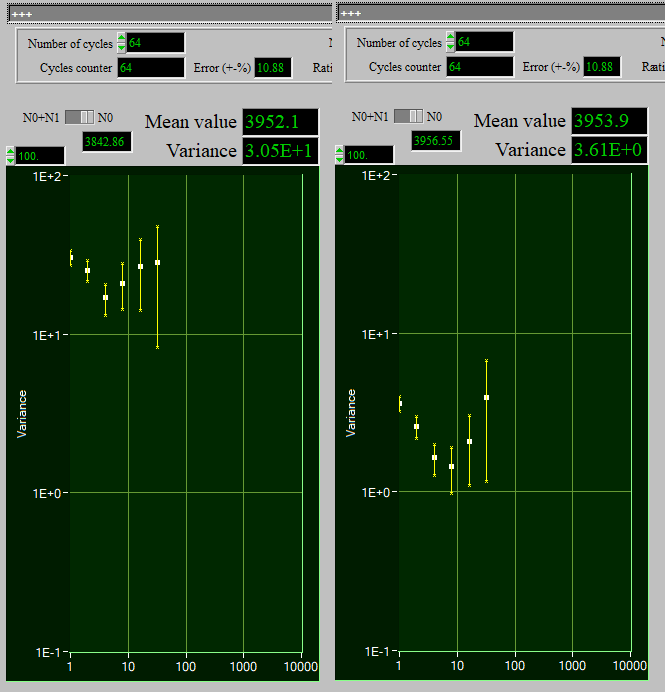
\includegraphics[width=0.4\linewidth]{figures/allan_averages.png}
    \caption{Desvios padrões de Allan sem (esquerda) e com (direita) o loop de estabilização de potência ativado.}
    \label{fig:allan}
\end{figure}

\begin{figure}
    \centering
    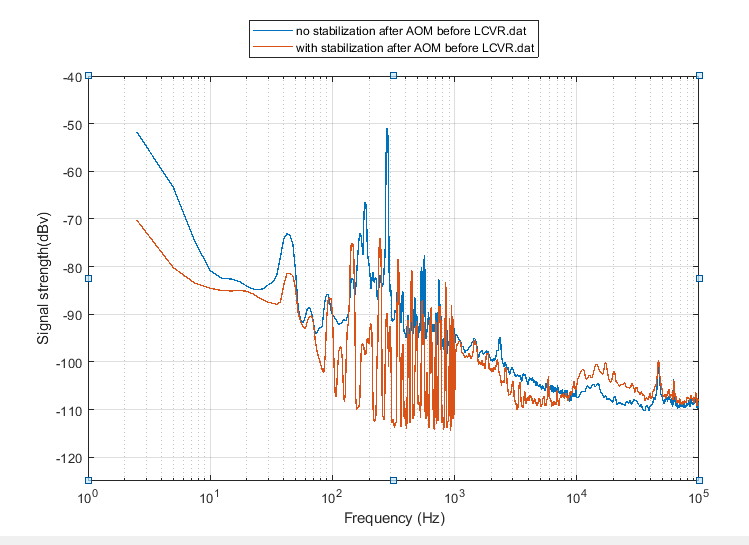
\includegraphics[width=0.5\linewidth]{figures/spectrum stabilization.png}
    \caption{FFT da parte AC da potência no fotodiodo Thorlabs posicionado após o \gls{AOM} com (laranja) e sem (azul) estabilização.}
    \label{fig:spectrum}
\end{figure}

\subsection{Oscilações de Rabi}
Realizamos algumas avaliações da frequência de Rabi para diferentes potências dos lasers Raman variando a amplitude do sinal RF enviado para o \gls{AOM} e o driver de corrente do TA, como pode ser visto na Tabela \ref{tab:rabi}.

\begin{table}[]
\begin{tabular}{{|p{2cm}|p{2cm}|p{2cm}|p{2cm}|}}
\hline
Amplitude do AOM (\si{V}) & Corrente do TA (\si{mA}) & Período do pulso de Pi (\si{\micro s}) & Frequência de Rabi (\si{kHz})                                      \\ \hline
0.1           & 1000           & 30                                                            & 16.7                                                                                \\ \hline
0.15          & 1000           & 17                                                            & 29.5                                                                                 \\ \hline
0.7           & 1000           & 14                                                            & 35.7                                                                              \\ \hline
0.3           & 1000           & 13                                                            & 38.5                                       \\ \hline
0.4           & 1200           & 10                                                            & 50                                                   \\ \hline
\end{tabular}
\caption{Frequências de Rabi em acoplamento co-propagante com diferentes voltagens de configuração do \gls{AOM}. A resposta do \gls{AOM} é não linear e atinge um platô em torno de \SI{0.3}{V}. Por isso, aumentamos a corrente do \gls{TA} no final.}
\label{tab:rabi}
\end{table}

\subsection{Interferometria de gravímetro}
Com um acoplamento contra-propagante e frequência de Rabi de \SI{35}{kHz} e, portanto, um pulso de $\pi/2$ de \SI{7}{\micro\second} e um pulso $\pi$ de \SI{14}{\micro\second}, realizamos um interferômetro com a configuração atual que foi capaz de fornecer o valor da gravidade. Para isso, usamos os três pulsos Raman conforme descrito acima. Além disso, aplicamos um chirp no desacordo entre os dois lasers Raman, de modo a compensar o desvio Doppler. Esse desacordo é controlado pelo loop de trava de fase. Esse chirp adiciona uma fase extra ao interferômetro correspondente a $2\pi a T^2$, onde $a$ é a taxa de chirp em Hz/s. Para diferentes tempos de interrogatório, escaneamos a taxa desse chirp, o que permite escanear a fase do interferômetro e, assim, observar franjas. Quanto maior o tempo de interrogatório, menor a distância entre as franjas, como em um interferômetro de Ramsey (ver fig. \ref{fig:gravi}). Para recuperar o valor da gravidade a partir disso, identificamos a taxa de chirp para a qual todos os padrões de franja apresentam um mínimo. Isso ocorre quando a taxa de chirp compensa exatamente a aceleração da queda dos átomos $g\cdot k_{eff}T^2$, o que significa que cancela a diferença de fase, independentemente do valor de $T$. Com a taxa de chirp de ressonância igual a $\approx \SI{-25.145}{MHz/s}$ obtida do ponto mais baixo nas franjas de 4000µs próximas à ressonância (novamente fig. \ref{fig:gravi}), podemos obter o valor da gravidade com $g k_{eff} = -2\pi a$, onde $k_{eff}=2\frac{2\pi}{780nm}$ e $a$ é a taxa de chirp de ressonância. O valor obtido de $g$ é igual a \SI{9.80655}{m/s^2}. Não chegamos ao limite da nossa precisão. Esta gravimetria foi mais uma validação das capacidades do sistema de laser Raman do que uma medição metrológica real.


\begin{figure}
    \centering
    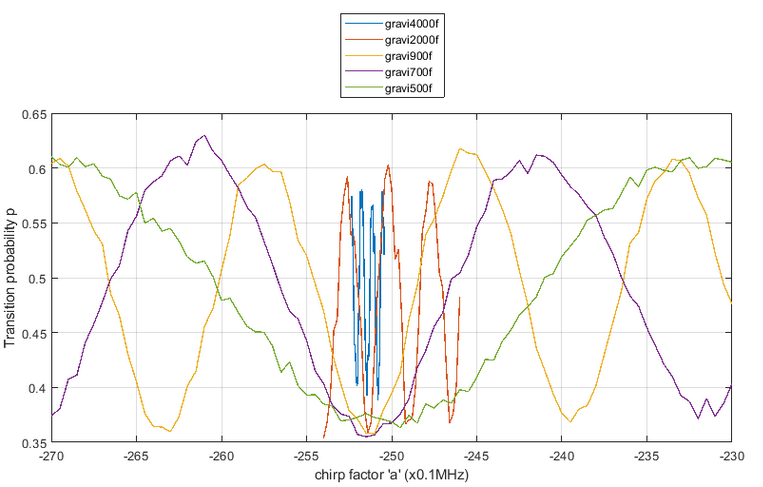
\includegraphics[width=0.7\linewidth]{figures/centralFringeGravimeter.PNG}
    \caption{Franjas de interferometria de átomos com um chirp de frequência aplicado à diferença de frequência entre os lasers Raman, para diferentes tempos de interrogatório $T$ em microssegundos. A variável escaneada foi a taxa de chirp escalada em \SI{0.1}{MHz/s}.
}
    
    \label{fig:gravi}
\end{figure}



\subsection{Discussão}

O \gls{TA} pareceu ser a escolha mais prática para obter uma potência maior para os lasers Raman. No entanto, o problema é a baixa qualidade do perfil do feixe que sai do \gls{TA}. Idealmente, deveríamos conseguir um acoplamento na fibra de cerca de \SI{50}{\percent}, mas só conseguimos cerca de metade disso, aproximadamente \SI{25}{\percent}. Para melhorar isso, poderíamos ter testado mais telescópios diferentes para tentar fazer com que o perfil do feixe de saída correspondesse melhor ao perfil ideal do feixe da fibra. O problema é que isso exigiria lentes com valores muito específicos e a tentativa de todas elas para otimizar o acoplamento ajustando a ampliação do telescópio.

Outra possível mudança seria tentar melhorar a posição do chip do amplificador para que o feixe saia alinhado ao eixo óptico, o que reduziria a aberração das lentes que colimam a saída do \gls{TA}. Essa mudança também melhoraria o acoplamento. Outra possibilidade seria escolher as lentes ideais para colimar a saída do \gls{TA} que corresponderiam diretamente ao perfil da fibra sem a necessidade de um telescópio. Mas isso nos levaria novamente ao problema de encontrar distâncias focais muito específicas para as lentes.
